\section{Problema 1 - \texorpdfstring{$M$}{M}-QAM}

\subsection{Introdução}
Na modulação,\textit{quadrature amplitude modulation} (QAM) os símbolos de informação são mapeados nas amplitudes das portadoras em fase e quadratura. Um modelo simplificado do sinal transmitido é visto como a equação~\ref{eq:QAM_coef}.
\begin{equation}
    s_m(t) = ( A_m^{(\text{real})} + j A_m^{(\text{imag})}) g(t)
    \label{eq:QAM_coef}
\end{equation}

No caso especial em que amplitudes $A_m^{(\text{real})}$ e $A_m^{(\text{imag})}$ assumem valores discretos no conjunto da equação~\ref{eq:QAM_retangular}, a constelação é chamada QAM retangular. O QAM retangular se aplica ao caso estudado a seguir, pois a quantidade de símbolos utilizados ($M = \{4, 16, 64\}$) se encaixam na condição e é utilizado para construção do alfabeto da modulação~\cite{Cecilio}. A função \href{https://raw.githubusercontent.com/lucasabdalah/Courses-HWs/SCD/Sistemas%20de%20Comunicacoes%20Digitais/matlab/problema1/const_MQAM.m}{\colorbox{cyan!10}{const\_MQAM.m}} foi

desenvolvida de modo a construir o alfabeto como uma matriz para ordenar os símbolos da esquerda para direita em linhas de símbolos ímpares e, da direita para esquerda em linhas pares.
\begin{equation}
    A_m = \{(2m -\sqrt{M} - 1)d \}_{m=1}^{\sqrt{M}}
    \label{eq:QAM_retangular}
\end{equation}


% ----------------------------------------------------------
\subsection{Energia da Constelação} 
Para calcular a energia média, é suficiente de calcular a equação~\ref{eq:E_media}, desenvolvida em \cite{Cecilio,Proakis}.
\begin{equation}
    \mathcal{E}_{media} = \frac{M-1}{3} \mathcal{E}_g
    \label{eq:E_media}
\end{equation}
Sendo $g(t)$ o pulso de energia unitária, $\mathcal{E}_g = 1$. O resultado é computado pela função função \href{https://raw.githubusercontent.com/lucasabdalah/Courses-HWs/SCD/Sistemas%20de%20Comunicacoes%20Digitais/matlab/problema1/energia_MQAM.m}{\colorbox{cyan!10}{energia\_MQAM.m}} para cada constelação QAM e é registrado na Tabela~\ref{tab:Resume_QAM}.

A relação entre $\mathcal{E}_{media} = \mathcal{E}_b \log_2{M}$ permite calcular diretamente a energia média de bit ($\mathcal{E}_b$), resultando na equação~\ref{eq:E_b}
\begin{equation}
    \mathcal{E}_b = \frac{M-1}{3\log_2 M} \mathcal{E}_{media}
    \label{eq:E_b}
\end{equation}
% ----------------------------------------------------------
\subsection{Distância Mínima entre Símbolos}
O parâmetro $d$ é a distância entre os símbolos adjacentes, e pode ser obtido com o cálculo da distância euclidiana entre estes, como na equação~\ref{eq:parametro_d}.
\begin{equation}
    \begin{split}
        d & = \sqrt{\frac{\mathcal{E}_g}{2}[(A_{mi} - A_{ni})^2 + (A_{mq} - A_{nq})^2]}\\
        & = \sqrt{\frac{3 \mathcal{E}_{media}}{2(M-1)}}
    \end{split}
    \label{eq:parametro_d}
\end{equation}
Essa distância é computada pela função \href{https://raw.githubusercontent.com/lucasabdalah/Courses-HWs/SCD/Sistemas%20de%20Comunicacoes%20Digitais/matlab/problema1/d_MQAM.m}{\colorbox{cyan!10}{d\_MQAM.m}} e registrada na Tabela~\ref{tab:Resume_QAM}.

\begin{table}[!ht]
    \centering
    \begin{tabular}{|c|c|c|c|}
        \hline
        $M$-QAM & $\mathcal{E}_{media}$ & $\mathcal{E}_{b}$ & $d$ \\ \hline
        & &  &  \\ 
        $M$ & $\frac{M-1}{3} \mathcal{E}_g$ & $ \frac{M-1}{3\log_2 M} \mathcal{E}_g$ & $\sqrt{\frac{3 \mathcal{E}_{media}}{2(M-1)}} $ \\ 
         &   &   &  \\ \hline
        $4$  & 1 & $1.67\times 10^{-1}$ & $\sqrt{2}/2$\\ \hline
        $16$ & 5 & $4.67\times 10^{-1}$ & $\sqrt{2}/2$\\ \hline
        $64$ & 21 & $1.17\times 10^{0}$ & $\sqrt{2}/2$\\ \hline
    \end{tabular}
    \caption{Informações gerais calculadas para a modulação $M$-QAM.}
    \label{tab:Resume_QAM}
\end{table}
\clearpage
% --------------------------------------------------------------
\subsection{Modulador (Codificação de Gray)}
O mapeador da constelação $M$-QAM consiste em uma função  que recebe uma sequência de bits e retorna o símbolo equivalente: \href{https://raw.githubusercontent.com/lucasabdalah/Courses-HWs/SCD/Sistemas%20de%20Comunicacoes%20Digitais/matlab/problema1/mapping_MQAM.m}{\colorbox{cyan!10}{mapping\_MQAM.m}}. Dentro desta função, é criado um alfabeto de código binário e na sequência ele é convertido convertido em Gray com \href{https://raw.githubusercontent.com/lucasabdalah/Courses-HWs/SCD/Sistemas%20de%20Comunicacoes%20Digitais/matlab/gray_const.m}{\colorbox{cyan!10}{gray\_const.m}}. 

Esta codificação é baseada em um algoritmo recursivo~\ref{alg:Gray}, cujo recebe uma sequência de bits orientadas pelo bit mais importante (MSB)~\cite{Gray}. A recursão está na operação ``ou exlusivo'' (\textit{xor}), denotada pelo símbolo $(\otimes)$. Este cálculo é executado na função \href{https://raw.githubusercontent.com/lucasabdalah/Courses-HWs/SCD/Sistemas%20de%20Comunicacoes%20Digitais/matlab/mybin2gray.m}{\colorbox{cyan!10}{mybin2gray.m}}.

% \clearpage

% global change
\SetKwInput{KwData}{Entrada}
\SetKwInput{KwResult}{Saída}

\begin{algorithm}[!ht]
    \SetAlgoLined
    \KwData{Sequência de Bits $(b)$ - MSB}
    \KwResult{Sequencia em Código Gray $(g)$ - LSB}
    $n = 0$\;
    $K = \text{length}(b)$\;
    \While{$K > n$}{
        \eIf{$K==n$}
        {$g_{(K-n)} = b_{(K-n)}$ \;}
        {$g_{(K-n)} = b_{(K-n+1)} \otimes b_{(K-n)}$\;}
        $n=n+1$;\;}
    $g = flip(g)$\;
    \caption{Codificação de Gray}
    \label{alg:Gray}
\end{algorithm}

Tabela~\ref{tab:Alfabeto_Gray} mostra um exemplo de conversão para código Gray de uma sequência de 2 bits. Seguindo o mesmo procedimento um alfabeto de qualquer tamanho pode ser criado.

\begin{table}[!ht]
    \centering
    \begin{tabular}{|c|c|c|c|}
        \hline
        Decimal & Binário & Gray & Decimal \\ \hline
        0 & 00 & 00 & 0\\ \hline
        1 & 01 & 01 & 1\\ \hline
        2 & 10 & 11 & 3\\ \hline
        3 & 11 & 10 & 2\\ \hline
    \end{tabular}
    \caption{Tabela de tradução de binário para Gray com 2 bits.}
    \label{tab:Alfabeto_Gray}
\end{table}

As constalações $M$-QAM para $M = \{4, 16, 64\}$ são apresentadas nas figuras~\ref{fig:4_QAM_plot}, \ref{fig:16_QAM_plot} e \ref{fig:64_QAM_plot}, respectivamente. É possível observar os valores dos símbolos em fase e quadratura, além do equivalente em binário.

\clearpage
\begin{figure}[!ht]
    \centering
    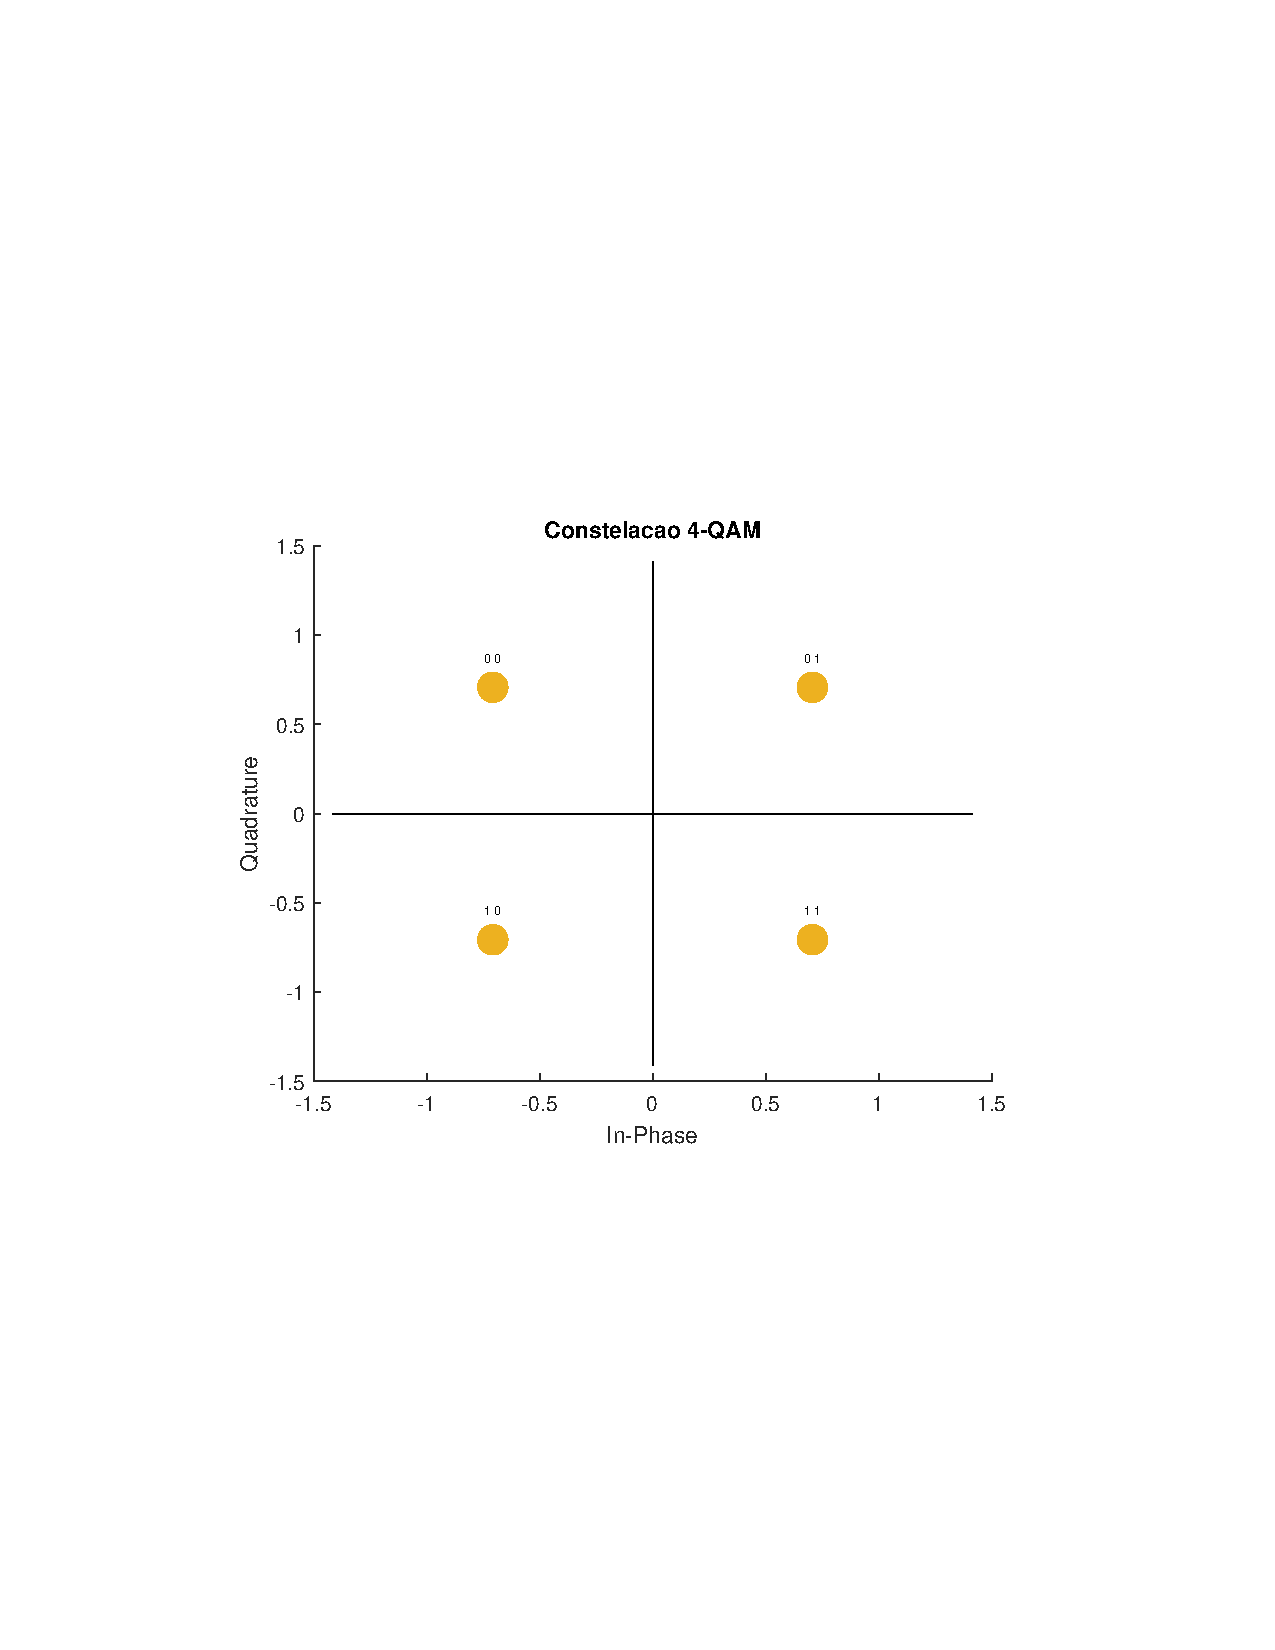
\includegraphics[width=1.0\textwidth,clip=true,trim={1.5cm 8.5cm 1.8cm 8.3cm}]{C:/Users/lukin/Documents/GitHub/Courses-HWs/Sistemas de Comunicacoes Digitais/matlab/problema1/fig/4_QAM_plot.pdf}
    \caption{Constelação 4-QAM plot.}
    \label{fig:4_QAM_plot}
\end{figure}

\begin{figure}[!ht]
    \centering
    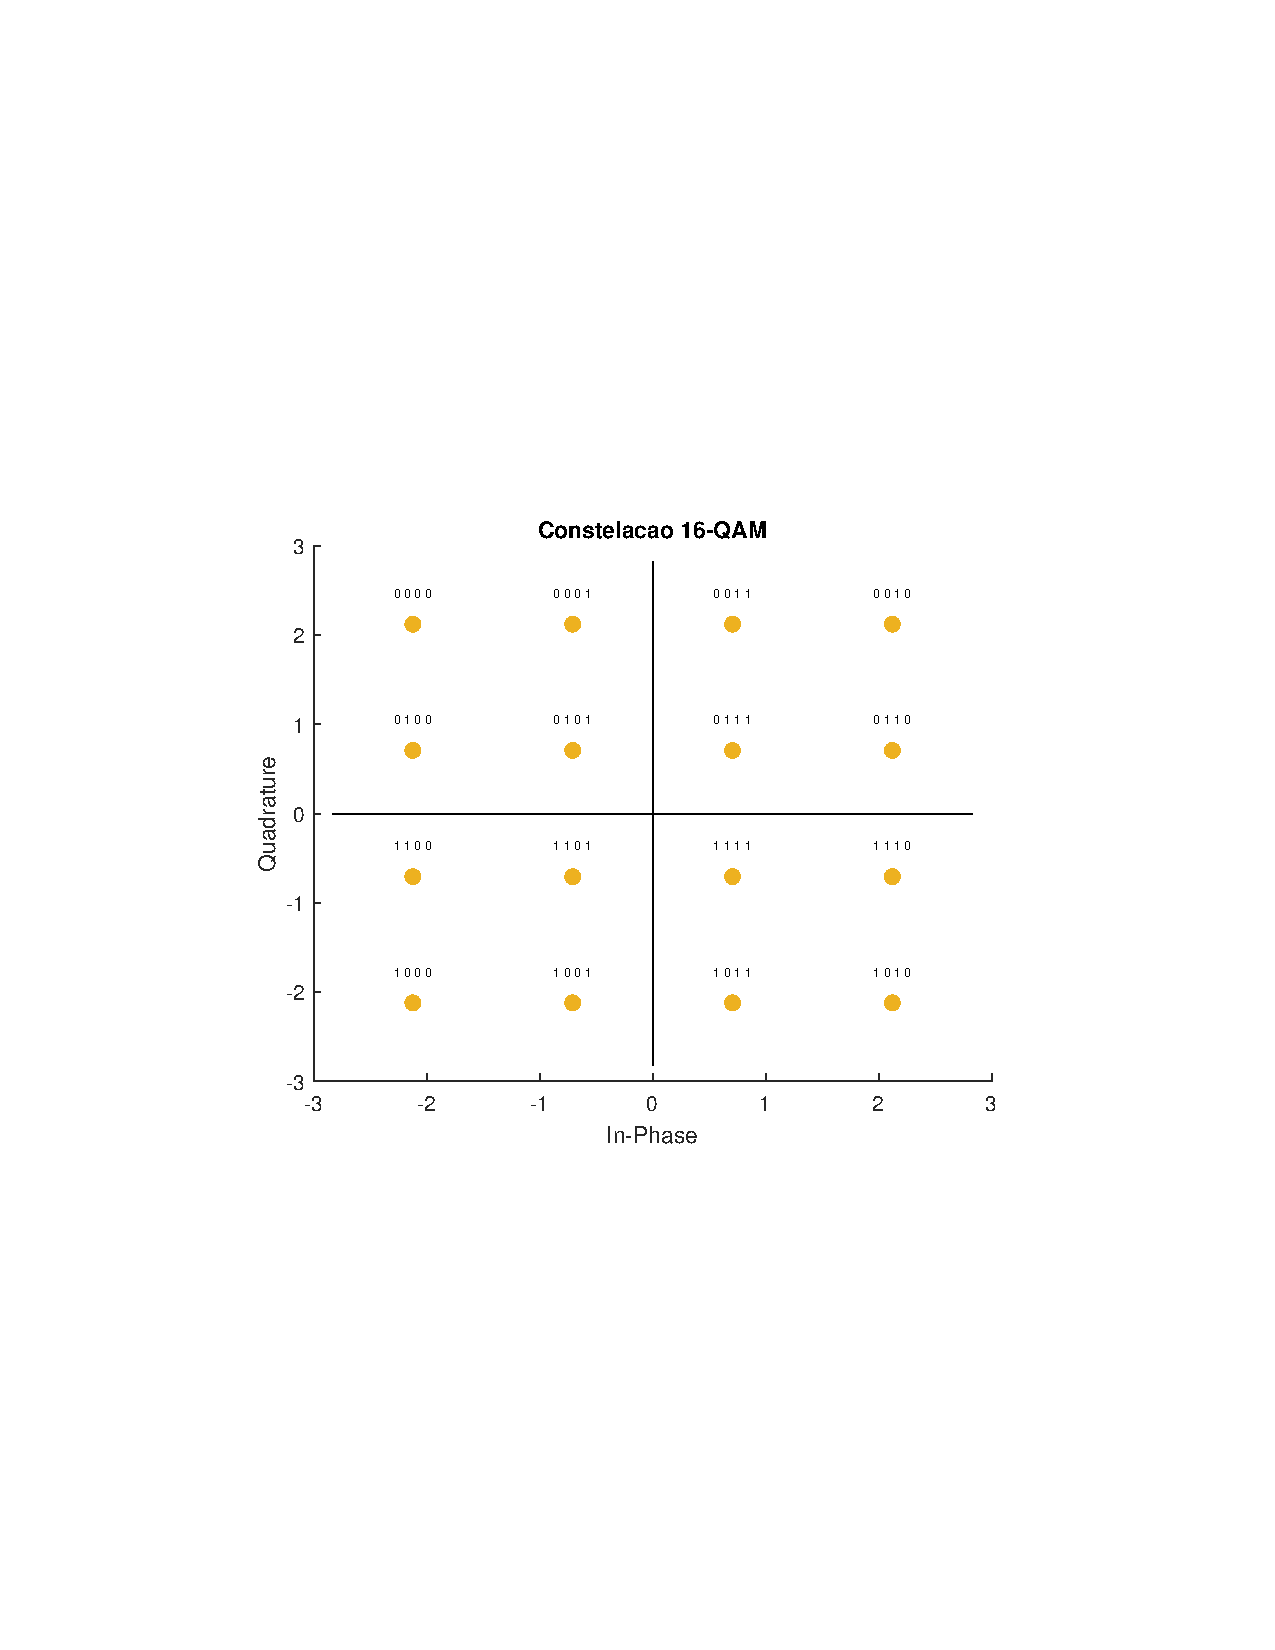
\includegraphics[width=1.0\textwidth,clip=true,trim={1.5cm 8.5cm 1.8cm 8.3cm}]{C:/Users/lukin/Documents/GitHub/Courses-HWs/Sistemas de Comunicacoes Digitais/matlab/problema1/fig/16_QAM_plot.pdf}
    \caption{Constelação 16-QAM plot.}
    \label{fig:16_QAM_plot}
\end{figure}

\clearpage

\begin{figure}[!ht]
    \centering
    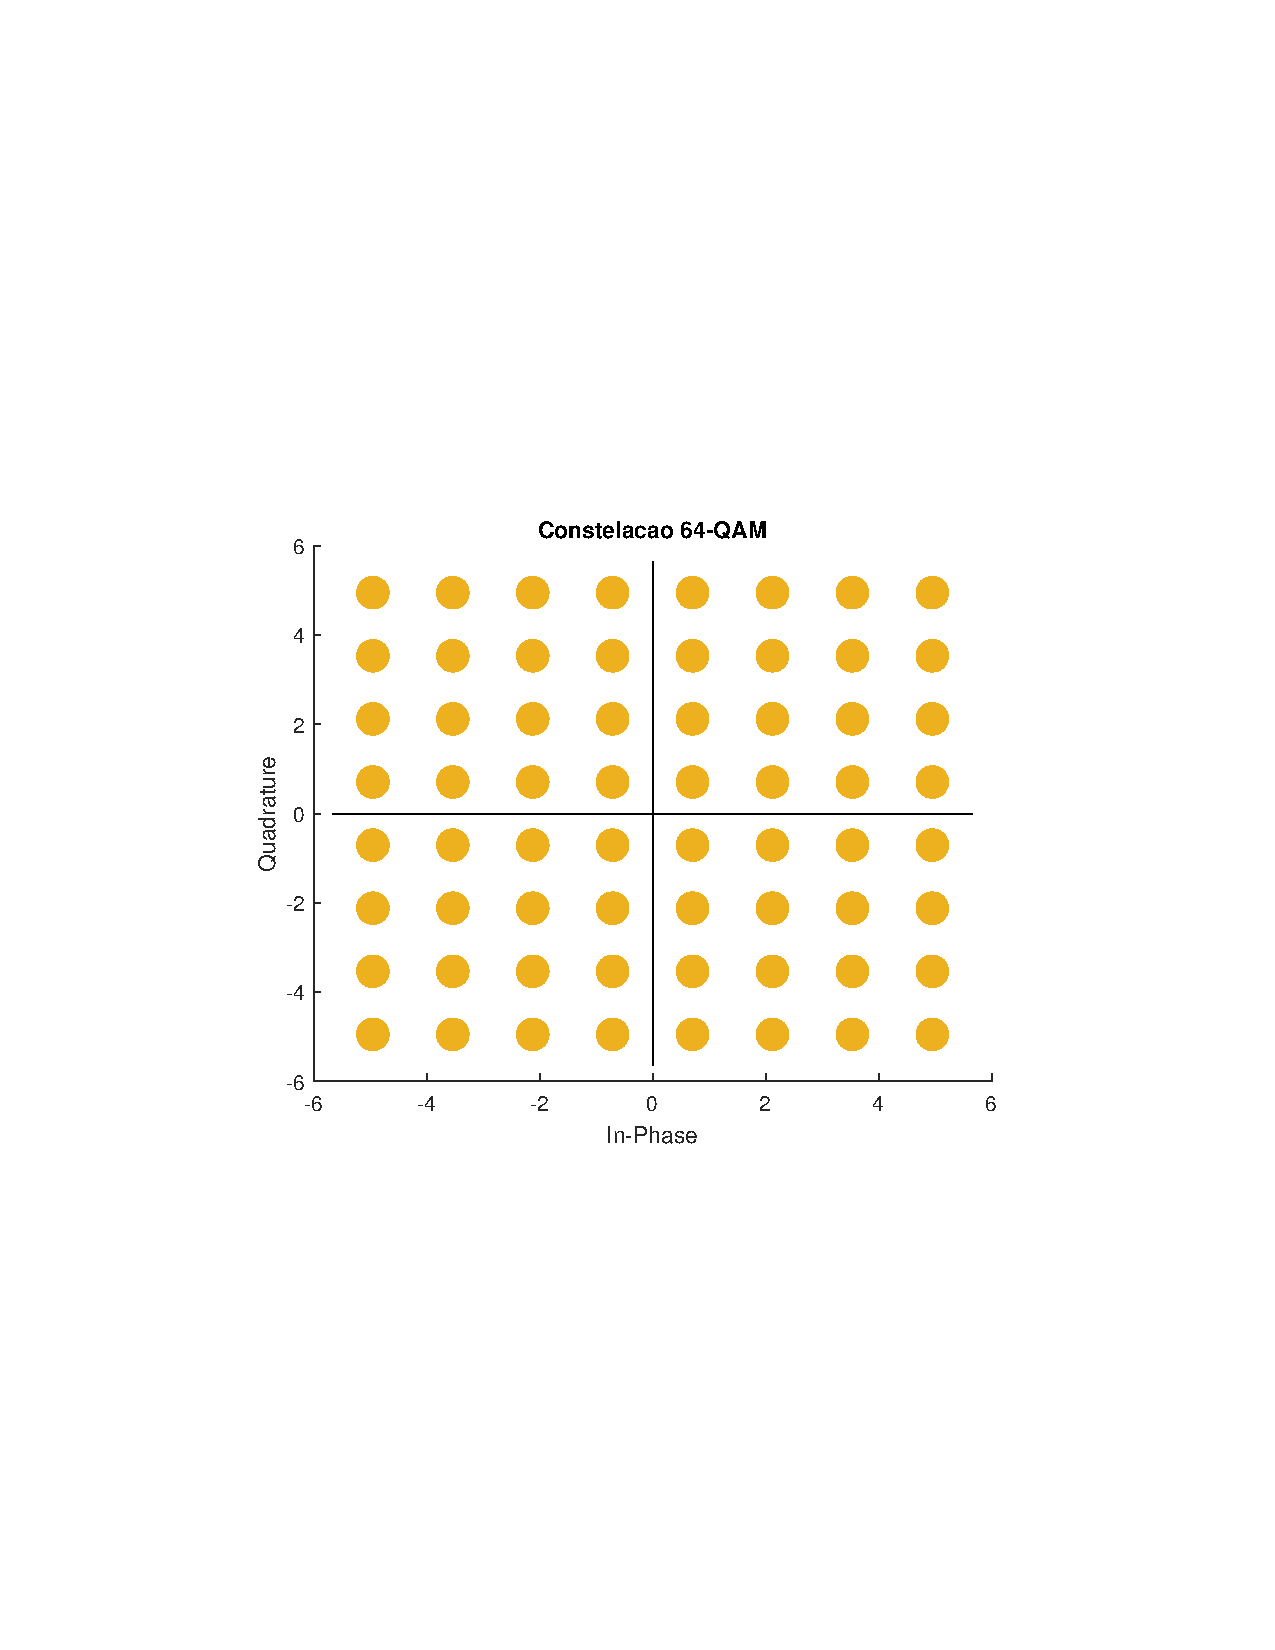
\includegraphics[width=1.0\textwidth,clip=true,trim={1.5cm 8.5cm 1.8cm 8.3cm}]{C:/Users/lukin/Documents/GitHub/Courses-HWs/Sistemas de Comunicacoes Digitais/matlab/problema1/fig/64_QAM_plot.pdf}
    \caption{Constelação 64-QAM plot.}
    \label{fig:64_QAM_plot}
\end{figure}

% --------------------------------------------------------------
\subsection{Demodulador}

A função que decodifica um símbolo tem como entrada o próprio símbolo: $A_n^{(\text{real})}$ e $A_n^{(\text{imag})}$, $M$ e $d$. 

O alfabeto da constelação $M$-QAM é gerada e uma vez estes definidos, a área de decisão é desenhada a partir em função de $M$ e $d$. Basicamente, o símbolo selecionado é aquele que minimiza a distância euclidiana entre o símbolo recebido e o do alfabeto, como mostra a equação~\ref{eq:dist_eucliadiana}.
\begin{equation}
    d_{mn} = \sqrt{|| s_m - s_n||^2}
    \label{eq:dist_eucliadiana}
\end{equation}

A função que executa estes comando é a \href{https://raw.githubusercontent.com/lucasabdalah/Courses-HWs/SCD/Sistemas%20de%20Comunicacoes%20Digitais/matlab/problema1/demapping_MQAM.m}{\colorbox{cyan!10}{demapping\_MQAM.m}} e ela retorna o símbolo decodificado e os bits equivalente do alfabeto de Gray. 

As figuras~\ref{fig:4_QAM_d_E} e \ref{fig:16_QAM_d_E} mostram uma geração de sequência de 50 símbolos aleatórios (\textit{i.i.d}) passando pelo demodulador com o traçado da distância euclidiana entre o símbolo recebido e o equivalente escolhido na constelação.

\clearpage 

\begin{figure}[!ht]
    \centering
    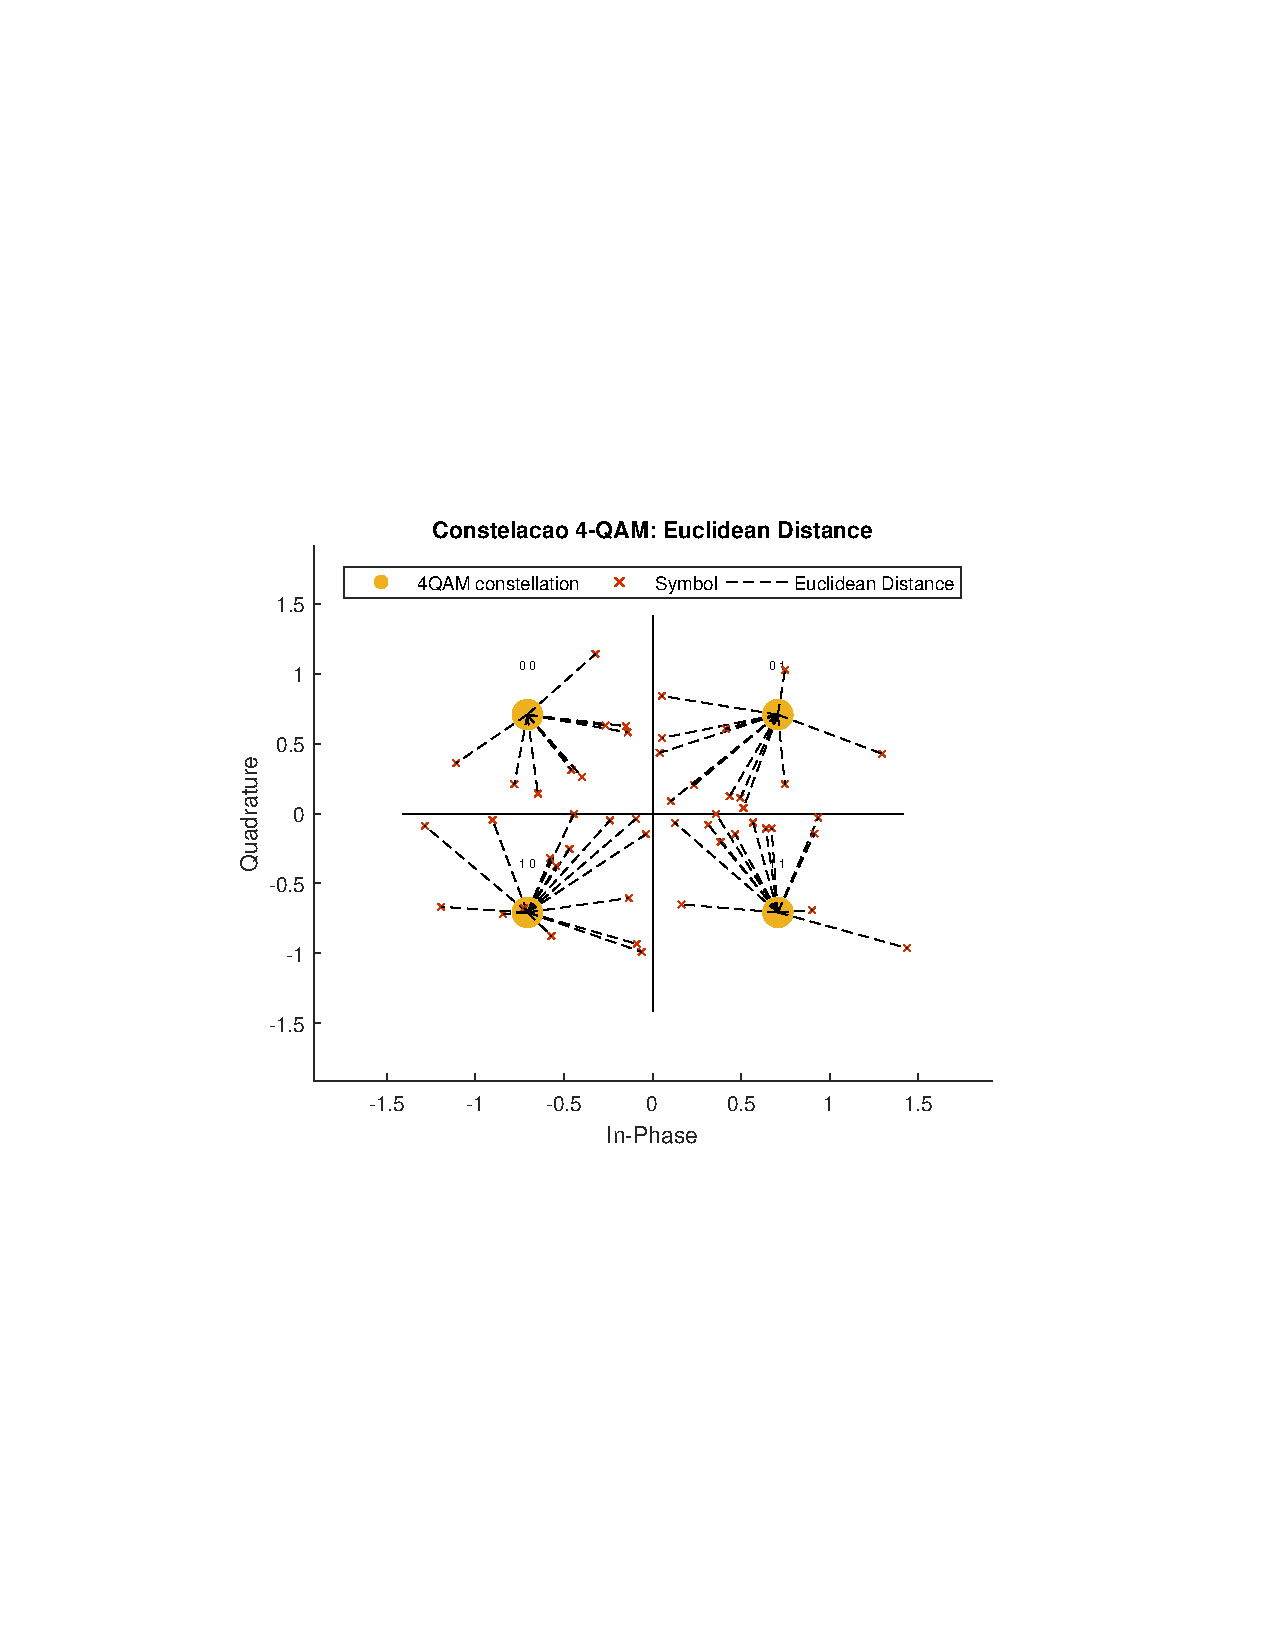
\includegraphics[width=1.0\textwidth,clip=true,trim={1.5cm 8.5cm 1.8cm 8.3cm}]{C:/Users/lukin/Documents/GitHub/Courses-HWs/Sistemas de Comunicacoes Digitais/matlab/problema1/fig/4example_QAM_plot.pdf}
    \caption{Exemplo de 4-QAM plot.}
    \label{fig:4_QAM_d_E}
\end{figure}

\begin{figure}[!ht]
    \centering
    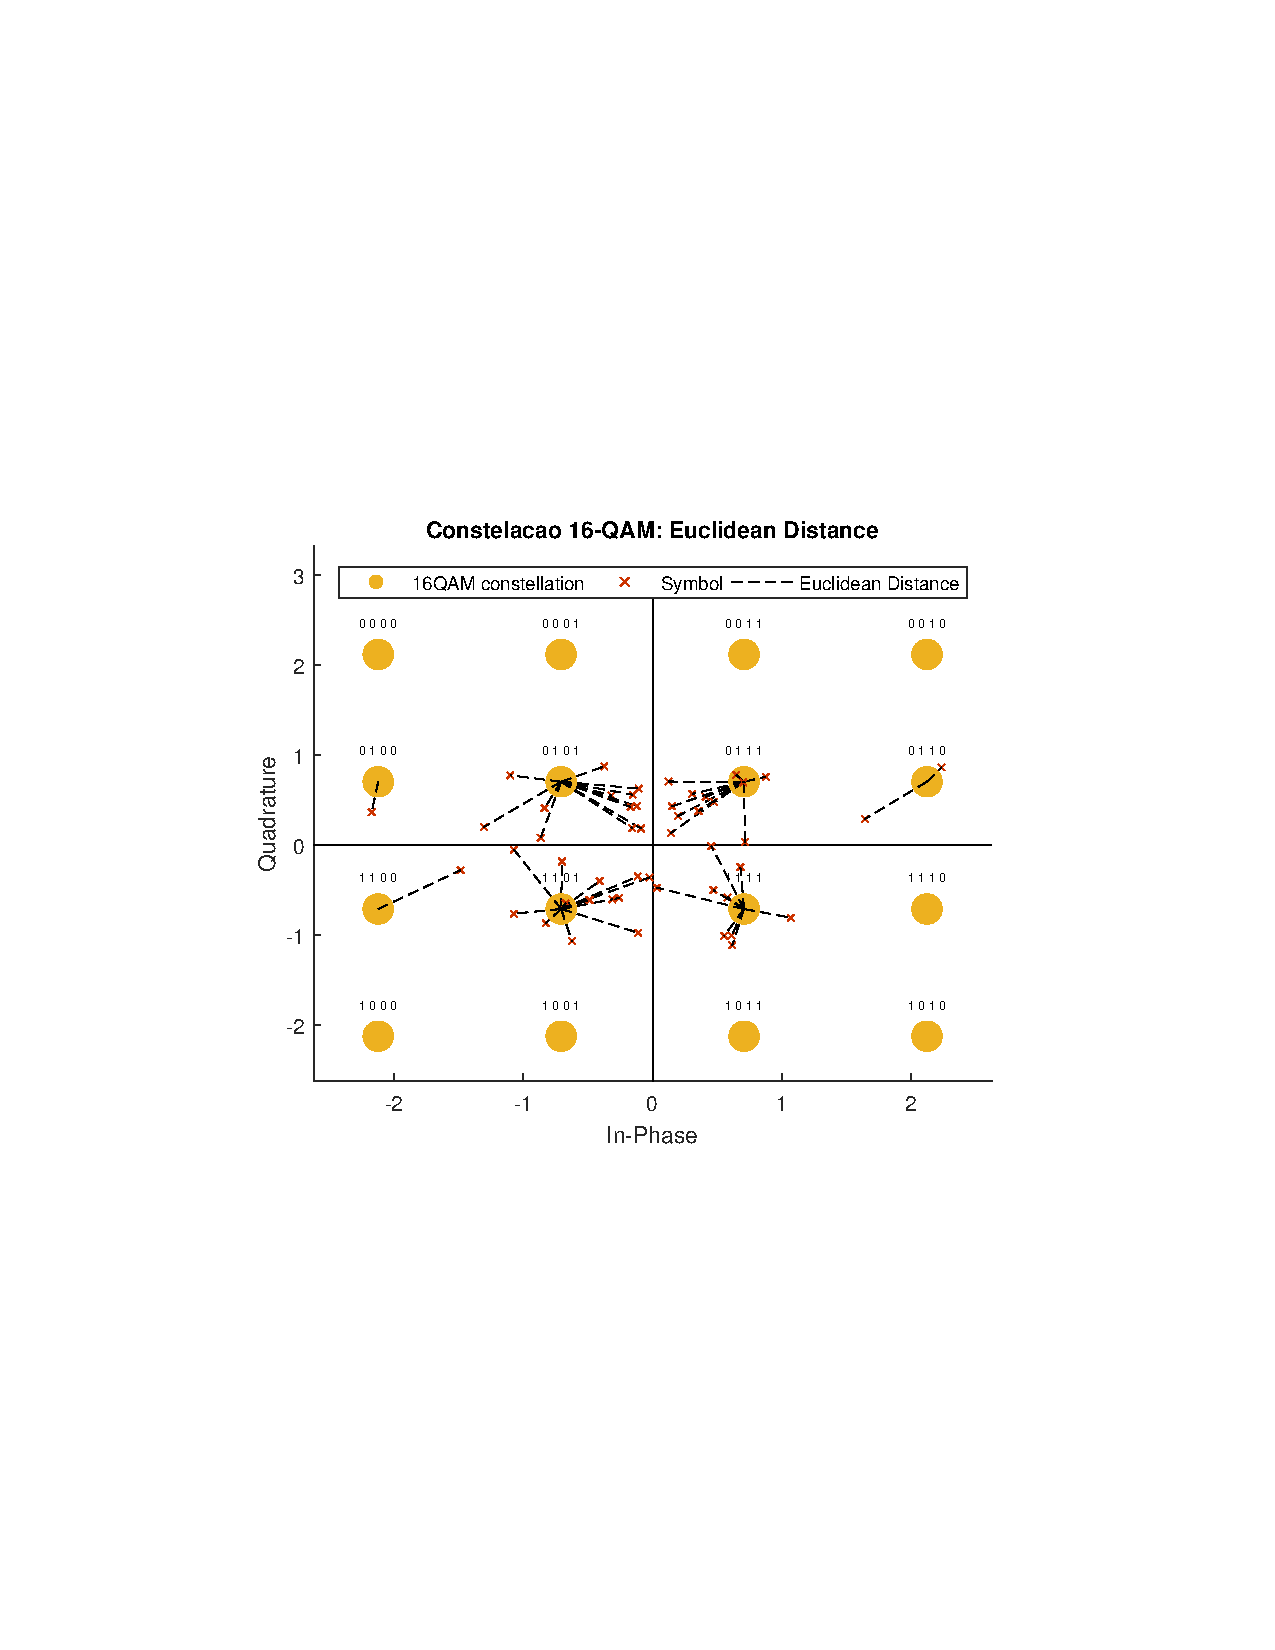
\includegraphics[width=1.0\textwidth,clip=true,trim={1.5cm 8.5cm 1.8cm 8.3cm}]{C:/Users/lukin/Documents/GitHub/Courses-HWs/Sistemas de Comunicacoes Digitais/matlab/problema1/fig/16example_QAM_plot.pdf}
    \caption{Exemplo de 16-QAM plot.}
    \label{fig:16_QAM_d_E}
\end{figure}